% ============================================================================
% main.tex  --  REVISED manuscript (effect-size vs evidence reframe)
% Canonical submission source. Legacy/overclaiming drafts are not part of this repo.
% ============================================================================
\pdfminorversion=7
\documentclass[11pt,a4paper]{article}

\usepackage[utf8]{inputenc}
\usepackage[T1]{fontenc}
\usepackage{lmodern}
\usepackage[protrusion=true,expansion=false]{microtype}
\usepackage[margin=2.5cm]{geometry}
\usepackage{graphicx}
\usepackage{booktabs}
\usepackage{siunitx}               % decimal-aligned numeric table columns
\sisetup{detect-all}
\usepackage{amsmath}
\usepackage{caption}
\usepackage[numbers,sort&compress]{natbib}
\usepackage{xcolor}
\usepackage[hidelinks]{hyperref}    % clickable but no coloured boxes around refs/cites
\usepackage{xurl}
\usepackage{setspace}
\usepackage{multirow}
\usepackage{lineno}                 % line numbers for review

\onehalfspacing                     % cleaner than double; still review-friendly
\emergencystretch=3em

% --- professional caption styling: bold "Table N.", smaller text ---
\captionsetup{labelfont={bf},font=small,labelsep=period}

\pagestyle{plain}                   % Arabic page numbers in the footer

% --- make lineno cooperate with amsmath display environments ---
\newcommand*\patchAmsMathEnvironmentForLineno[1]{%
  \expandafter\let\csname old#1\expandafter\endcsname\csname #1\endcsname
  \expandafter\let\csname oldend#1\expandafter\endcsname\csname end#1\endcsname
  \renewenvironment{#1}%
    {\linenomath\csname old#1\endcsname}%
    {\csname oldend#1\endcsname\endlinenomath}}%
\newcommand*\patchBothAmsMathEnvironmentsForLineno[1]{%
  \patchAmsMathEnvironmentForLineno{#1}%
  \patchAmsMathEnvironmentForLineno{#1*}}%
\AtBeginDocument{%
  \patchBothAmsMathEnvironmentsForLineno{equation}%
  \patchBothAmsMathEnvironmentsForLineno{align}%
  \patchBothAmsMathEnvironmentsForLineno{gather}%
  \patchBothAmsMathEnvironmentsForLineno{multline}}

\newcommand{\papertitle}{Separating effect size from statistical evidence in network-proximity rankings under target-count asymmetry: a controlled liver-interactome audit}
\title{\papertitle}

\date{}
\newcommand{\suppauthor}{Antony Bevan, Sarputheen M, and Vijayakumar Thangavel Mahalingam}

\begin{document}

\begingroup
\setlength{\parindent}{0pt}
\raggedright
{\Large\bfseries \papertitle\par}
\vspace{0.9em}
{\large Antony Bevan$^{1}$, Sarputheen M$^{2}$, and Vijayakumar Thangavel Mahalingam$^{2,*}$\par}
\vspace{0.7em}
{\small
$^1$Department of Pharmacognosy, Madurai Medical College, Madurai, India\par
$^2$Department of Pharmacy Practice, SRM College of Pharmacy, Faculty of Medicine and Health Science, SRM Institute of Science and Technology, Kattankulathur, Chennai, India\par
$^*$Corresponding author: Vijayakumar Thangavel Mahalingam; Email: \href{mailto:vijayakm2@srmist.edu.in}{vijayakm2@srmist.edu.in}\par
}
\vspace{1.8em}
\endgroup
\linenumbers

\section*{Abstract}

Network-proximity Z-scores are often compared across candidate compounds, but unequal target counts change the null variance of the averaged distance statistic. In a liver-expressed STRING interactome, we show that the null standard deviation shrinks approximately as $|T|^{-1/2}$, so standardized evidence can rank a larger target set above a smaller set even when its raw closest-distance effect is weaker. Hyperforin (10 targets) is closer to the drug-induced liver injury (DILI) module than Quercetin (62 targets) ($d_c = 1.30$ vs $1.68$, STRING $\geq$900) yet has the weaker proximity Z-score ($-3.86$ vs $-5.44$); the Z-score ordering also reverses between STRING thresholds while the raw-distance ordering does not. A degree-controlled calibration benchmark reproduces the same null-precision law across the DILI module and matched pseudo-modules, placing material rank reversal in a narrow, high-margin regime rather than as a generic outcome. As a complementary effect-size readout, perturbation efficiency (mean per-target influence) separates direct target--DILI overlap from propagated random-walk influence: 62\% of Hyperforin's efficiency is direct overlap, leaving a modest propagated advantage ($\sim$1.5$\times$). Target-asymmetric network comparisons should therefore report raw effect size, standardized evidence, and direct versus propagated influence separately.

\vspace{0.5em}
\noindent\textbf{Keywords:} network medicine; network proximity; proximity Z-score; target-count asymmetry; effect size; random walk with restart; drug-induced liver injury.


\section{Introduction}

% P1: The known
Network-based drug prioritization maps compound targets onto the human interactome and scores their proximity to disease-associated protein modules \citep{Hopkins2008, Barabasi2011, Menche2015, Guney2016}. The field standard, the proximity Z-score, calibrates each compound against a size- and degree-matched null and answers the question: is this compound unusually close to this disease? Guney et al.\ \citep{Guney2016} validated this Z-score as a per-pair classifier across 402 known drug--disease associations (mean 3.5 targets per drug) and showed that, within each drug's own null, the standardization removes the dependence that raw distance has on target count and degree.

% P2: The gap
Comparing Z-score \textit{magnitudes} across compounds, however, introduces a distinct requirement: the Z-score must be monotone in the underlying topological effect. When target counts differ sharply, the larger set's null standard deviation shrinks as $|T|^{-1/2}$---a consequence of the law of large numbers on an averaged statistic---so a compound with weaker raw proximity can register stronger standardized evidence. The American Statistical Association emphasizes that statistical significance ``does not measure the size of an effect or the importance of a result'' \citep{Wasserstein2016}, and whether this non-monotonicity materializes in network-medicine practice, and under what conditions, has not been systematically examined.

% P3: Our approach
We address this with a controlled stress test in a liver-expressed interactome. We select two \textit{Hypericum perforatum} constituents---Hyperforin (10 targets) and Quercetin (62 targets)---as a deliberately high-contrast diagnostic pair. Hyperforin is the PXR-activating, CYP-inducing constituent responsible for St John's Wort's clinically important hepatic drug--drug interactions \citep{Moore2000, Watkins2001, Chen2022}, making it a mechanistically motivated comparator for engagement of the DILI module's xenobiotic-metabolism axis; Quercetin provides the high-target-count comparator. The drug-induced liver injury (DILI) module serves as the disease reference, chosen because its inclusion of cytochrome-P450, transporter, and nuclear-receptor genes ---genes central to xenobiotic metabolism, transport, and regulatory response---exposes a second question: when does direct target--disease overlap inflate apparent network influence? We complement the pair with a degree-controlled calibration benchmark ($20{,}000$ probes per size, $500{,}000$ cross-size pairs) that characterizes the operating regime in which rank reversal can occur, and we introduce perturbation efficiency---mean per-target random-walk influence on the disease module---as a complementary effect-size measure. Target provenance, botanical context, and chemical-similarity controls are detailed in Methods and \S\ref{subsec:chemsim}.

% P4: What we found (roadmap)
We show that proximity Z-score magnitude and raw closest distance can dissociate under target-count asymmetry, trace this to the $|T|^{-1/2}$ null-precision law, and confirm that the law holds across shortest-path, random-walk, and expression-weighted influence alike. A degree-controlled liver-network benchmark reveals that material rank reversal is a located, conditional outcome---rare for generic target sets, realized when the smaller set is above the 90th percentile of probe-pair margins. On the diagnostic pair, perturbation efficiency ranks the PXR/CYP-inducing constituent higher while the direct--propagated decomposition exposes the direct target--DILI overlap that an uncritical headline number would have conflated with propagated influence. This is a controlled audit of how size-dependent null precision affects the interpretation of network-proximity rankings, not a DILI-prediction model.

\section{Results}

\subsection{The null standard deviation shrinks with target count for every metric}

The null standard deviation of the proximity Z-score follows a general property of averaged statistics: it shrinks as the number of targets grows. Drawing degree-matched random seed sets of increasing size and measuring the null standard deviation of per-target influence, we find $\sigma_{\text{null}} \propto |T|^{-0.48}$ (log--log slope; theoretical $-1/2$; Table~\ref{tab:scaling}); the degree-controlled benchmark of \S\ref{subsec:opregime} refines this exponent to $-0.499$ (95\% CI $[-0.502,-0.495]$). This is the Law of Large Numbers acting on a mean over targets, and it is observed across all three evaluated metrics: in the compound-specific degree-matched permutation nulls, the Hyperforin-to-Quercetin null-SD ratio is 2.40--2.57 for shortest-path, 2.45--3.04 for random-walk influence, and 2.47--2.93 for expression-weighted influence, against the expected $\sqrt{62/10} = 2.49$ (per-metric null parameters in Table~\ref{tab:s_nullsd}). For shortest-path the ratio brackets $\sqrt{62/10}$ within finite-$n$ estimation error ($n=1{,}000$); for random-walk and expression-weighted influence it runs somewhat higher (up to $3.04$), consistent with the heavier-tailed, degree-sensitive nulls of diffusion-based statistics \citep{Cowen2017, Erten2011}, whose standard deviations are estimated with larger finite-$n$ error. The $|T|^{-1/2}$ scaling itself is confirmed independently by the degree-controlled benchmark ($-0.499$), not by these per-metric ratios. Influence-based Z-scores are therefore subject to the same shrinkage as proximity Z-scores, and Z-score magnitude should not be interpreted as a direct effect-size comparison across compounds of very different target count; this is why we pair the evidence with an explicit effect size. We first characterize the operating regime in which the null-precision law produces rank reversal.

\begin{table}[ht]
\centering
\caption{\textbf{Null standard deviation of per-target influence scales as $|T|^{-1/2}$} (STRING $\geq$900; degree-matched random seed sets). The log--log slope is $-0.48$.}
\label{tab:scaling}
\begin{tabular}{@{}lccccc@{}}
\toprule
$|T|$ & 5 & 10 & 20 & 40 & 62 \\
\midrule
$\sigma_{\text{null}}$ & 0.0093 & 0.0068 & 0.0059 & 0.0035 & 0.0028 \\
\bottomrule
\end{tabular}
\end{table}



\subsection{The null-precision law defines a conditional operating regime for rank reversal}
\label{subsec:opregime}

To characterize the operating regime of the proximity Z-score under target-count asymmetry, we constructed a degree-controlled calibration benchmark on the same liver LCC and DILI module, sampling random target-set ``probes'' across sizes ($|T| \in \{5,8,10,15,20,30,40,60,62,80\}$) and comparing their raw closest distance with a size-level calibration Z-score; no toxicity outcome is modeled (Methods; \texttt{scripts/run\_operating\_regime\_benchmark.py}). This benchmark Z-score is used to study the operating behavior of standardization across target counts; it is not the per-compound Guney null used for the real compounds.

The null-precision mechanism is also observed in size-matched pseudo-module controls. The null standard deviation scales as $\sigma_{\text{null}} \propto |T|^{-0.499}$ (95\% CI $[-0.502,-0.495]$, $R^2=0.9999$; degree-distribution-pinned probes on a ten-point size grid, consistent with the coarser per-target-influence estimate of Table~\ref{tab:scaling}), indistinguishable from the theoretical $-1/2$ and from a uniform-probe control ($-0.500$), and the exponent is similar for the real DILI module ($-0.495$) and for random size-matched pseudo-modules ($-0.498$; Fig.~\ref{fig:opregime}A). The larger set's sharper null therefore gives it the \emph{capacity} to register weaker absolute proximity as stronger standardized evidence: the maximum raw-distance margin it can overturn is $\delta_{\max}(R) = (\mu_L-\mu_S) + |z_S|\,\sigma_L(\sqrt{R}-1)$ (Fig.~\ref{fig:opregime}B; this follows by solving $Z_L = Z_S$ for the raw margin $\delta = d_c^L - d_c^S$, using $\sigma_S/\sigma_L = \sqrt{R}$ from the $|T|^{-1/2}$ law). The variance contrast scales as $\sqrt{R}$; for a fixed smaller-set size, the overturnable raw-margin term can be written as $|z_S|\sigma_S(1-R^{-1/2})$, so it increases with target-count ratio but saturates. The coefficients are empirical: here the null-mean offset $\mu_L-\mu_S$ is negligible ($+0.001$), a property of this interactome's distance geometry rather than a structural zero.

Realized reversals are conditional. Using descriptive material-margin cutoffs for the smaller set's raw-distance advantage ($\geq 0.3$ hops, approximately $0.3/2.2 \approx 14\%$ of the null-mean closest distance in this network; $\geq 0.5$ hops, $\sim$23\%, as a stricter alternative), the larger set overturns the ranking in $\approx 0\%$ of degree-matched probe pairs up to $R=4$ and only $0.39\%$ at $R=8$ ($\geq 0.5$ hops: $\leq 0.01\%$ throughout; a no-shrinkage counterfactual gives $0\%$; Table~\ref{tab:s_opregime}). Unconditionally, however, Z-score and raw-distance rankings disagree in $\sim$12\% of cross-size comparisons at $R=6.2$, a rate that is non-negligible for naive cross-compound Z-score comparison. In this benchmark, material reversals are concentrated when the smaller set is above the 90th percentile of probe-pair margins (large $|z_S|$), so that a modest raw advantage falls under the $\delta_{\max}$ envelope. A biologically interpretable pair falling within this regime is examined next (\S\ref{subsec:dissociate}).



\subsection{Raw proximity and proximity-Z rank the two compounds differently}
\label{subsec:dissociate}

The Hyperforin/Quercetin pair falls within the characterized regime. Hyperforin's closeness margin over Quercetin ($d_c$ difference $0.38$) sits at the $91$st percentile of probe-pair margins and below the $\delta_{\max}\approx 0.63$ envelope at $R=6.2$, placing it inside the reversal region (Fig.~\ref{fig:opregime}C). In the liver-expressed largest connected component (LCC) of the STRING $\geq$900 interactome (7{,}677 nodes; 66{,}908 edges), Hyperforin engages 10 targets and Quercetin 62; the drug-induced liver injury (DILI) module contains 82 genes (Fig.~\ref{fig:context}; the 82-gene set is listed in Table~\ref{tab:s_dili}). Hyperforin's targets are topologically closer to the DILI module by shortest-path distance than Quercetin's, $d_c = 1.30$ versus $1.68$. The degree-matched proximity Z-scores order the compounds in the opposite direction: Hyperforin $Z = -3.86$, Quercetin $Z = -5.44$ (Table~\ref{tab:effevid}).

The Z-score is a standardized quantity, $Z = (d_c - \mu_{\text{null}})/\sigma_{\text{null}}$, in which the observed distance is compared to the mean and spread of distances for random target sets of the same size and degree. These two statistics answer different questions: $d_c$ measures raw topological effect; $Z$ measures standardized evidence against a null. Quercetin's 62 targets sit far below the tightly concentrated null expected for 62 random degree-matched genes ($\mu = 2.17$, $\sigma = 0.091$), producing a large $|Z|$; Hyperforin's 10 targets sit below a broader null ($\mu = 2.21$, $\sigma = 0.235$), producing a smaller $|Z|$ despite a shorter absolute distance. Hyperforin has the stronger raw closest-distance ($d_c$) effect; Quercetin has the stronger standardized evidence (Fig.~\ref{fig:dumbbell}). The instability is in the cross-compound \textit{evidence ranking}: between thresholds the proximity-Z ranking reverses (Hyperforin $Z = -6.04$ vs Quercetin $-5.46$ at $\geq$700; the order flips at $\geq$900), whereas the raw $d_c$ ranking (Hyperforin closer at both thresholds) does not.

\begin{table}[ht]
\centering
\caption{\textbf{Effect size and standardized evidence dissociate under target-count asymmetry} (STRING $\geq$900). Hyperforin is closer ($d_c$) yet less ``significant'' ($Z$); the difference is driven by the smaller null standard deviation of the larger target set.}
\label{tab:effevid}
\begin{tabular}{@{}l S[table-format=2.0] S[table-format=1.2] S[table-format=1.2] S[table-format=1.3] S[table-format=-1.2]@{}}
\toprule
\textbf{Compound} & {\textbf{$n$ targets}} & {\textbf{$d_c$}} & {\textbf{$\mu_{\text{null}}$}} & {\textbf{$\sigma_{\text{null}}$}} & {\textbf{$Z$}} \\
\midrule
Hyperforin & 10 & 1.30 & 2.21 & 0.235 & -3.86 \\
Quercetin  & 62 & 1.68 & 2.17 & 0.091 & -5.44 \\
\bottomrule
\end{tabular}
\end{table}



\subsection{Perturbation efficiency is the mean per-target influence}

We quantify influence with random walk with restart (RWR) \citep{Kohler2008, Cowen2017}. With column-normalized transition matrix $W = AD^{-1}$, restart probability $\alpha$, and restart vector $\mathbf{p}_0$, let $\mathbf{I}_n$ denote the $n \times n$ identity matrix. The steady state is
\begin{equation}
\mathbf{p} = \alpha\,[\,\mathbf{I}_n - (1-\alpha)W\,]^{-1}\mathbf{p}_0. \label{eq:rwr}
\end{equation}
Influence on the DILI module $D$ is
\begin{equation}
I(T,D) = \sum_{d \in D} p_d. \label{eq:infl}
\end{equation}
Taking the restart vector uniform over the target set, $p_0(i) = 1/|T|$ for $i \in T$ and $0$ otherwise, Eq.~\eqref{eq:rwr} is linear in $\mathbf{p}_0$, so
\begin{equation}
E(T,D) \equiv I(T,D) = \frac{1}{|T|}\sum_{t \in T}\sum_{d \in D} p_d^{(t)}, \label{eq:pe}
\end{equation}
Perturbation efficiency $E$ is therefore exactly the mean per-target influence on the disease module --- a size-normalized effect-size measure, not a re-standardized evidence statistic. Here $\mathbf{p}^{(t)}$ denotes the RWR steady-state vector seeded from target $t$ alone. We verified Eq.~\eqref{eq:pe} numerically (joint vs mean-of-single-target influence agree to RWR tolerance: $0.11380975$ vs $0.11380968$ for Hyperforin).

At STRING $\geq$900, $E = 0.1138$ for Hyperforin and $0.0322$ for Quercetin (Fig.~\ref{fig:efficiency}; and $0.1212$ vs $0.0326$ at $\geq$700): unlike the proximity-Z ranking, which reverses between thresholds (\S\ref{subsec:dissociate}), the per-target influence ranking is stable across the two evaluated network thresholds for both RWR and expression-weighted influence (Table~\ref{tab:s_threshold}). The ranking is robust to the restart probability across $\alpha \in [0.10, 0.70]$ (Hyperforin above Quercetin throughout), although the magnitude of the ratio is $\alpha$-dependent (2.90 at $\alpha=0.10$ to 13.35 at $\alpha=0.70$; Table~\ref{tab:s_alpha}); we therefore treat the ranking, not the ratio, as the robust feature, and do not interpret $\alpha$-sensitive fold ratios as absolute biological constants. Expression weighting (destination-node liver expression; Methods) preserves the ordering (Fig.~\ref{fig:ewi}) and is insensitive to the expression floor (efficiency ratio 2.69--2.70 across floors $0$--$0.1$; Table~\ref{tab:s_floor}).


\subsection{Separating direct overlap from propagated influence}

The raw per-target advantage ($3.5\times$) conflates two mechanistically distinct contributions. We isolate the propagated component and then stress-test it through a chain of controls: an orthogonal separation measure, per-target distance-1 connectivity, removal of the overlapping module genes, and a size-matched bootstrap. Four of ten Hyperforin targets (ABCB1, CYP2C9, MMP2, NR1I2) are themselves DILI-module genes (Tables~\ref{tab:s_evidence}, \ref{tab:s_hyptargets}), versus one of sixty-two for Quercetin (MMP2), so part of Hyperforin's measured disease-module influence is \emph{direct}: steady-state probability assigned to seed nodes that are themselves DILI-module genes. The canonical proximity framework retains such distance-zero contributions, treating a drug target that coincides with a disease protein as a real, if special, signal \citep{Guney2016}; we retain it likewise, but separate it from indirect, network-\emph{propagated} influence. Analogous to leave-one-out scoring used in network propagation \citep{Kohler2008, Cowen2017}, we score each target against the disease module \emph{excluding the target itself}, isolating the propagated part of the module influence (Eq.~\eqref{eq:infl}).

Decomposed this way (Table~\ref{tab:leakage}, Fig.~\ref{fig:leakage}), 62\% of Hyperforin's per-target influence is direct overlap (direct component $0.0711$ versus $0.0032$ for Quercetin, only 10\% of which is direct), while its propagated component is $0.0427$ versus $0.0290$, a propagated advantage of $1.5\times$ that is far below the raw $3.5\times$. The propagated component remains above a degree-matched background: it sits at the 99.9th percentile of a degree-matched random 10-gene background ($n=1{,}000$; $3.3\times$ the background mean, empirical $p=0.002$), although it does not exceed every random set, and some size-matched Quercetin subsets reach comparable values; alternative exclusions of the propagated term bound the advantage to $1.2$--$1.9\times$. Both components concentrate in the PXR--CYP--transporter axis, which is at once the established mechanism of Hyperforin-mediated hepatic interactions and the locus of the overlap. The propagated advantage is therefore modest, layered on a larger and mechanistically coherent direct-overlap effect rather than reflecting a clear topological separation. Two further topology checks clarify this interpretation: the network separation measure $S_{AB}$ \citep{Menche2015} shows both target sets are topologically separated from the DILI module, Hyperforin slightly more so (Table~\ref{tab:s_sep}). This does not contradict the $d_c$ result because $S_{AB}$ also depends on within-set compactness; Hyperforin's target set is tighter internally ($\langle d_{AA}\rangle = 1.20$ vs $1.55$), raising its separation despite its shorter closest distance. Separately, Hyperforin's targets carry more direct (distance-1) DILI connections per target (3.4 vs 1.5; Table~\ref{tab:s_connectivity}), so the advantage is concentrated in a few directly DILI-linked targets. The decomposition is also robust to the disease-module definition itself: removing the four entangled pharmacogenes from the module, so the targets cannot directly overlap it, leaves the propagated advantage intact and marginally larger ($1.47\times \to 1.58\times$; Table~\ref{tab:s_modulesens}), showing the propagated residual is not eliminated when direct overlap is removed from the module. A size-matched bootstrap of the raw influence (Fig.~\ref{fig:bootstrap}) reproduces the baseline ratio but, lacking the overlap adjustment, is superseded by this decomposition.

\begin{table}[ht]
\centering
\caption{\textbf{Direct versus propagated decomposition of per-target influence} (STRING $\geq$900). Raw influence separates into a direct component (steady-state mass on target$\cap$DILI nodes, retained following \citet{Guney2016}) and a propagated component isolated by leave-one-out \citep{Kohler2008}; alternative exclusions of the propagated term bound the residual advantage. The direct-overlap ratio is reported descriptively and is not interpreted as a biological fold-effect.}
\label{tab:leakage}
\begin{tabular}{@{}l S[table-format=1.4] S[table-format=1.4] S[table-format=2.1]@{}}
\toprule
\textbf{Component / control} & {\textbf{$E$(Hyperforin)}} & {\textbf{$E$(Quercetin)}} & {\textbf{ratio}} \\
\midrule
Raw per-target influence & 0.1138 & 0.0322 & 3.5 \\
\quad Mass on target$\cap$DILI nodes & 0.0711 & 0.0032 & 22.5 \\
\quad Propagated (leave-one-out) & 0.0427 & 0.0290 & 1.5 \\
\midrule
Propagated, CYP/transporter targets removed & 0.0338 & 0.0290 & 1.2 \\
Propagated, shared targets removed & 0.0541 & 0.0288 & 1.9 \\
\bottomrule
\end{tabular}
\end{table}


\subsection{The proximity computation is faithful to the canonical implementation}

We next compared the proximity result against Guney et al.'s canonical toolbox implementation: the closest distance reproduces exactly (observed $d_c$ 1.300/1.677) and the Z-scores to within permutation tolerance. All reference distributions use $n=1{,}000$ random sets, fixed seed 42, Guney's $\geq$100-node degree-binning, and preserve the DILI module size ($|D|=82$). Under the fixed-disease null (randomizing targets only, disease module held at the 82 DILI genes), the $\geq$100-node binning gives Hyperforin $Z = -4.09$, Quercetin $Z = -5.34$ --- Quercetin more ``significant'' despite being topologically farther by shortest-path distance. Under Guney's two-sided null (randomizing both the target set and a degree-matched disease set of size 82), both compounds remain strongly proximal relative to their nulls but the dissociation attenuates to near-parity: Hyperforin $Z = -3.55$, Quercetin $Z = -3.66$ (the null standard deviation continues to shrink with set size, ratio 2.37 vs expected 2.49). The interpretation is consistent: Hyperforin is the topologically closer compound in every construction, while its evidence ranking relative to Quercetin depends on the null --- strongest when the actual DILI module is held fixed, the configuration relevant to comparing two compounds against one disease (Table~\ref{tab:guney}).

\begin{table}[ht]
\centering
\caption{\textbf{Revalidation against the canonical proximity implementation} (STRING $\geq$900, $n=1{,}000$, seed 42, $\geq$100-node degree-binning, $|D|=82$ preserved). The effect/evidence dissociation is clear under the fixed-disease null and attenuates under the two-sided null; Hyperforin is the closer compound throughout. The raw $d_c$ ordering (Hyperforin closer) is invariant across all constructions; the $Z$-score evidence difference is null-dependent.}
\label{tab:guney}
\begin{tabular}{@{}l S[table-format=-1.2] S[table-format=-1.2]@{}}
\toprule
\textbf{Null model ($d_c$)} & {\textbf{Hyperforin $Z$}} & {\textbf{Quercetin $Z$}} \\
\midrule
Repo $\pm$25\% window, fixed disease (primary) & -3.86 & -5.44 \\
Guney $\geq$100-bin, fixed disease & -4.09 & -5.34 \\
Guney $\geq$100-bin, two-sided & -3.55 & -3.66 \\
\bottomrule
\end{tabular}
\end{table}


\subsection{Chemical-similarity specificity control}
\label{subsec:chemsim}

Neither compound is a close structural analogue of DILIrank 2.0 reference drugs \citep{Chen2016, Olubamiwa2025}---the retrievable-SMILES binary subset of DILIrank 2.0 (542 DILI-positive, vMost/vLess-concern, and 365 DILI-negative, vNo-concern, drugs; the 354 ambiguous-concern drugs are excluded; Methods)---with maximum Tanimoto to any DILIrank reference drug $<0.4$ (Hyperforin 0.20, Quercetin 0.22; the maxima against DILI-positive references alone are 0.15 and 0.21 \citep{Maggiora2014}), so structural-analogue similarity to those compounds is unlikely to explain the observed network pattern (Fig.~\ref{fig:chemsim}); this argues against close structural-analogue confounding within the DILIrank reference set.

\section{Discussion}

Our results build on the proximity framework established by Guney et al.\ \citep{Guney2016}: the proximity Z-score is a calibrated \textit{evidence} statistic---each compound is compared to a size- and degree-matched null, and a larger target set legitimately yields sharper significance. The phenomenon we characterize arises when the task shifts from per-compound classification to cross-compound ranking. Under target-count asymmetry, Z-score \textit{magnitude} should not be read as a biological effect-size ordering. Because the Z-score's denominator shrinks as $|T|^{-1/2}$ (a property we confirm for shortest-path, random-walk, and expression-weighted influence alike), the evidence ranking can diverge from, and even reverse, the raw topological effect ranking. This is the established distinction between effect size and statistical significance emphasized by the American Statistical Association \citep{Wasserstein2016}, here in a network-medicine setting.

The practical recommendation is to report both the evidence Z-score and an explicit effect size. We use per-target random-walk influence (perturbation efficiency), which by linearity of the walk equals the mean single-target influence on the disease module and is therefore comparable across compounds with unequal target counts. This metric complements the Z-score rather than replacing it: it does not itself escape variance shrinkage at the level of its own Z-score. Random-walk influence is also sensitive to node degree \citep{Cowen2017, Erten2011}, which is one reason we decompose it into direct-overlap and propagated components below.

Perturbation efficiency ranks Hyperforin above Quercetin, consistent with its xenobiotic-metabolism biology; Hyperforin is the PXR/CYP-inducing constituent mechanistically linked to DILI-relevant bioactivation \citep{Moore2000, Watkins2001, Chen2022}. This ordering holds across restart-probability variation, network threshold, and degree-binning. Decomposing the advantage, however, shows that it is largely \emph{direct} target--disease overlap: 62\% of Hyperforin's per-target influence comes from four targets that are themselves DILI-module genes. The \emph{propagated} component, isolated by leave-one-out, is a modest $1.5\times$ (about $1.2$--$1.9\times$ across alternative exclusions); its distribution overlaps size-matched Quercetin subsets, though it remains above a degree-matched background. Both components concentrate in the xenobiotic-metabolism axis that defines the mechanism and the overlap alike. Hyperforin's propagated advantage is above a degree-matched background (99.9th percentile, $3.3\times$ the mean) and above the mean of size-matched Quercetin subsets, while still overlapping their upper tail; the direct-overlap component is mechanistically interpretable but not independent evidence of propagated network positioning.

\subsection{Relationship to prior work}

Our findings build on Guney et al.'s proximity framework \citep{Guney2016} by identifying a cross-compound ranking regime that the original per-pair study design did not stress-test. Guney et al.\ evaluated proximity as a per-pair classifier across 238 drugs and 78 diseases (402 known drug--disease associations; mean 3.5 targets per drug), and demonstrated that the closest-distance relative proximity is essentially uncorrelated with target degree ($\rho=-0.01$); that is a statement about classification calibration within each drug's own size-matched null, not about the comparability of Z-\textit{magnitudes} across compounds whose target counts differ several-fold. Our task is different: cross-compound ranking under extreme target-count asymmetry (10 vs 62). In that regime the size-dependence of the null standard deviation, which the per-pair Z-score calibrates through its null mean and null variance, re-emerges when Z-magnitudes are compared between compounds. The resolution is not a new significance statistic but the separate reporting of effect size, for which per-target influence is a natural choice. Random walk with restart is conceptually adjacent to attenuated-distance and diffusion-style measures, but it is not identical to Guney's diffusion-kernel proximity ($d_k$), which downweights longer \emph{shortest paths} by an exponential penalty rather than propagating restart-anchored probability mass over the adjacency matrix; we therefore do not use Guney's $d_k$ result to argue for or against random-walk influence. The choice between proximity measures is orthogonal to our argument: a normalized influence measure can define an effect-size scale that should be reported \emph{alongside} the standardized evidence rather than in place of it when compounds of unequal size are compared. Degree bias in network propagation and prioritization is well documented \citep{Erten2011, Cowen2017, Barel2020}; the operating-regime benchmark (\S\ref{subsec:opregime}) complements node-degree control by explicitly calibrating the target-count axis, establishing that the $|T|^{-1/2}$ null-precision law is stable across the DILI module and size-matched pseudo-modules and that the resulting effect/evidence reversal is a \emph{located, conditional} regime — one that materializes when the smaller target set is above the 90th percentile of probe-pair margins.

\subsection{Limitations}

This study is a controlled two-compound audit designed to characterize the statistical behavior of proximity Z-scores under target-count asymmetry; it does not evaluate toxicological outcomes or predict DILI. Hyperforin is not an established intrinsic hepatotoxin \citep{LiverToxSJW}; the pair was selected for target-count contrast and mechanistic interpretability. Network influence is a measure of topological reach, not a toxicological outcome: it omits dose, exposure, pharmacokinetics, binding directionality (agonism vs antagonism), and reactivity. The two target sets also differ in provenance, not only size: Hyperforin's ten targets are literature-curated and mechanistically central (the PXR receptor with its induced enzymes and transporters), whereas Quercetin's sixty-two are a broad ChEMBL bioactivity net (Table~\ref{tab:s_evidence}). This evidentiary asymmetry could in principle contribute to Hyperforin's apparent advantage independently of topology; the direct--propagated decomposition and the DILI-module sensitivity (Table~\ref{tab:s_modulesens}) are designed to bound that confound (the propagated advantage survives both), but they do not eliminate it, and a fully curation-matched comparison would require harmonized target evidence for both compounds, which we note as a limitation. The ChEMBL-derived Quercetin target set may also include assay-context targets that differ from clinically relevant exposure targets. Generalization to compound libraries, for example testing whether perturbation efficiency carries DILI signal beyond target count and degree across DILIrank 2.0 with curated target sets, is a direction for future work. The operating-regime benchmark (\S\ref{subsec:opregime}) establishes that the $|T|^{-1/2}$ exponent is stable across the DILI module and size-matched pseudo-modules and that the reversal is a located, conditional regime; the \emph{rate} of reversal depends on the module's distance geometry and would differ in other networks. Its probes are degree-controlled random sets rather than curated drug-target sets, so it characterizes the statistic, not a drug population. Finally, interactome incompleteness and degree bias in random-walk propagation \citep{Cowen2017, Erten2011} bound the precision of all network-based statements made here.

\subsection{Conclusion}

Network-proximity Z-scores are valid evidence statistics whose magnitude should not be read as a cross-compound effect-size ranking under target-count asymmetry. Reporting raw effect size, standardized evidence, and per-target influence decomposed into direct-overlap and propagated components separately yields a more transparent comparative picture. A degree-controlled liver-network calibration shows that the null-precision law is stable across the DILI module and size-matched pseudo-modules, and that material rank reversal is a conditional regime requiring a smaller target set above the 90th percentile of probe-pair margins. In the worked example, the framework ranks the PXR/CYP-inducing constituent higher while exposing and separating out the direct target--disease overlap that an uncritical headline number would have conflated with propagated influence.

\section{Methods}

\subsection{Interactome and modules}
Human protein functional associations were obtained from the STRING v12.0 functional association network \citep{Szklarczyk2023} (combined score integrating experimental, curated-database, co-expression, genomic-context, and text-mining channels; we use ``interactome'' in this broad association-network sense, not as a purely physical binding network) at combined-confidence $\geq$900, mapped to HUGO gene symbols, and filtered to genes with GTEx v8 liver median TPM $\geq$1 \citep{GTEx2020}; the largest connected component (LCC) was retained using NetworkX \citep{Hagberg2008} (7{,}677 nodes, 66{,}908 edges, from a raw $\geq$900 STRING network of 11{,}693 nodes / 100{,}383 edges; the $\geq$700 network, 9{,}773 LCC nodes, is used for threshold robustness). DILI-associated genes were obtained from DisGeNET curated associations (UMLS C0860207) \citep{Pinero2020}, giving 82 genes in the $\geq$900 LCC; this is a curated association module, not a validated causal gene set. Hyperforin targets (10 in the LCC) were curated from primary literature \citep{Moore2000, Watkins2001, Obach2000, Komoroski2004, Hennessy2002, Assefa2004, Wang2004, Quiney2007, Quiney2006}; Quercetin targets (62 in the LCC) were assembled from ChEMBL-derived bioactivity records \citep{Mendez2019} (the programmatic retrieval is documented in the repository's data manifest rather than re-executed here; see Data Availability). Protein identifiers were mapped to HUGO symbols via UniProt \citep{UniProt2023}, with non-human proteins excluded and symbols standardized (e.g.\ MDR1$\rightarrow$ABCB1); raw counts (14 Hyperforin, 122 Quercetin) reduce to 10 and 62 in the LCC (Table~\ref{tab:s_curation}). Five genes are targeted by both compounds (ABCG2, AKT1, CYP3A4, MMP2, MMP9) and are retained in both sets; four further literature-reported Hyperforin targets (TRPC6, VEGFA, PMAIP1, GRIN1) fall outside the liver-expressed LCC and are not analyzed \citep{Leuner2007, Hostanska2003, Kumar2006}.

\subsection{Closest distance and proximity Z-score}
Closest distance is the mean shortest path from each target to the nearest disease-module gene \citep{Guney2016}:
\begin{equation}
d_c(T,D) = \frac{1}{|T|}\sum_{t\in T}\min_{s\in D}\mathrm{dist}(t,s).
\label{eq:dc}
\end{equation}
The proximity Z-score standardizes this raw distance against a degree-matched null:
\begin{equation}
Z = \frac{d_c - \mu_{\text{null}}}{\sigma_{\text{null}}},
\label{eq:proxz}
\end{equation}
with $Z=0$ when $\sigma_{\text{null}}=0$. We use $n=1{,}000$ degree-matched random reference sets, fixed seed 42. Following Guney et al.\ \citep{Guney2016} we report $Z$ as the primary magnitude; we additionally report empirical, directional permutation p-values using the conservative $(r+1)/(n+1)$ convention \citep{Phipson2010} --- one-sided for smaller-than-null distance (proximity) and larger-than-null influence (RWR/EWI) --- whose floor at $n=1{,}000$ is $9.99\times10^{-4}$ (reported as $p<0.001$). For both compounds, $p<0.001$ confirms non-random proximity to the DILI module but does not discriminate between them; the Z-score is the primary comparative statistic. No two-tailed permutation p-value is used. Degree matching is performed both with a $\pm$25\% degree window (primary) and with Guney's $\geq$100-node degree-binning; the degree-binning choice has minimal effect under the fixed-disease null (Table~\ref{tab:s_guney}). In the Guney-fidelity comparison, we use random seed 42 rather than the toolbox default (452456), and the local shortest-path comparison sampler permits the original seed node in its own candidate pool whereas the toolbox excludes it; this is a $\leq$1\% candidate-pool difference for bins of $\geq$100 nodes, and the resulting Z-scores are unchanged within permutation tolerance (Table~\ref{tab:s_guney}). The shared RWR/EWI permutation sampler excludes original targets from the random candidate pool. The fixed-disease null (randomizing targets only) is primary, as it corresponds to comparing two compounds against one disease module; the two-sided null (randomizing both targets and disease, as in the canonical implementation) is reported as a robustness check.

\subsection{Random walk with restart and perturbation efficiency}
RWR uses $W=AD^{-1}$, restart $\alpha=0.15$ (a PageRank-style damping value; the canonical RWR reference is K\"ohler et al.\ \citep{Kohler2008}, where $\alpha$ is typically larger and results are reported robust to it; Guney et al.\ \citep{Guney2016} use shortest-path proximity and define no restart parameter), convergence tolerance $10^{-6}$, and $\leq$100 iterations. Influence and perturbation efficiency are defined by Eqs.~\eqref{eq:rwr}--\eqref{eq:pe}; perturbation efficiency equals mean per-target influence by linearity of the steady state in the restart vector. Degree-matched permutation nulls ($n=1{,}000$, seed 42) provide influence Z-scores and empirical p-values; Benjamini--Hochberg correction is applied within each network threshold. A full restart-probability sweep ($\alpha\in[0.10,0.70]$) is reported.

\subsection{Expression weighting}
Transitions are weighted by destination-node liver expression, $W'_{ij} = A_{ij} e_i / \sum_k A_{kj} e_k$, with $e_i$ the min--max-normalized $\log_2(\mathrm{TPM}+1)$ from GTEx v8 liver \citep{GTEx2020}; an expression floor of 0.01 maintains reachability and is shown to be immaterial (floor sweep $0$--$0.1$).

\subsection{Direct--propagated decomposition}
To separate direct target--disease overlap from propagated influence we isolate the propagated component by leave-one-out (scoring each target against the module excluding the target itself, thereby excluding the disease-member seed's own contribution from its module score) and report the following controls: removal of DILI-member seeds; removal of cytochrome-P450/transporter seeds; removal of targets shared by both compounds; comparison to global degree-matched random 10-gene sets; and size-matched Quercetin subsets. The network separation measure $S_{AB}$ \citep{Menche2015} is reported as an orthogonal overlap statistic. As a network-construction robustness check, we additionally rebuilt the interactome excluding STRING edges supported solely by text mining \citep{Huang2018} and re-ran all metrics, arguing against text-mining-only edges as the driver of the observed effect ordering (Supplementary Note, \textit{Text-mining robustness}).

\subsection{Chemical similarity}
Morgan fingerprints (ECFP4; radius 2, 2048 bits) were generated with RDKit \citep{RDKit2023}; maximum Tanimoto similarity to DILIrank 2.0 reference drugs \citep{Chen2016, Olubamiwa2025} was computed, with 0.4 as the structural-analogue threshold \citep{Maggiora2014}. DILIrank 2.0 classifies 1{,}336 drugs into four concern categories; we used the binary subset with retrievable PubChem SMILES, mapping vMost- and vLess-DILI-concern to DILI-positive (542 drugs) and vNo-DILI-concern to DILI-negative (365 drugs), and excluding the ambiguous-DILI-concern category.

\subsection{Operating-regime benchmark}
To assess whether the statistical mechanism underlying the effect-size/evidence dissociation extends beyond the worked pair, we sampled random target-set probes on a ten-point size grid ($|T|=5$--$80$, including the observed 10- and 62-target sizes; 20{,}000 probes per size) from the liver LCC and computed each probe's closest distance to the DILI module and its size-level calibration Z-score. Primary probes were degree-distribution-pinned to the full compound-target row degree profile (10 Hyperforin rows plus 62 Quercetin rows) using Guney's $\geq$100-node bins: for each probe, degree-bin labels were sampled with replacement from this target-row degree-bin distribution, and nodes were then sampled from the corresponding bins after excluding DILI-module genes from the candidate pool so distance-zero mass cannot scale with $|T|$. A non-DILI-target-profile family and a uniform-from-pool family were used as contrasts. The null parameters ($\mu_{\text{null}}$, $\sigma_{\text{null}}$) are estimated once per (size, degree-profile) family from the 20{,}000-probe reference distribution itself; each probe's calibration Z-score is its deviation from that shared size-level reference, not a separate per-probe permutation null. Because $N=20{,}000$, self-inclusion has negligible influence on size-level null parameters. We fitted the null-SD scaling exponent (log--log, bootstrap CI) and compared it across the DILI module and three random size-matched pseudo-modules. Rank discordance was quantified on cross-size probe pairs (500{,}000 per size pair; smaller set fixed at $|T|=10$): the maximum overturnable raw margin $\delta_{\max}(R)=(\mu_L-\mu_S)+|z_S|\,\sigma_L(\sqrt{R}-1)$, and the margin-conditional reversal rate (fraction of pairs in which the smaller set is closer by $\geq\delta_0$ hops yet the larger set has the more negative calibration Z-score) for pre-specified descriptive cutoffs $\delta_0\in\{0.3,0.5\}$, with a no-shrinkage ($\sigma_L:=\sigma_S$) counterfactual. These $\delta_0$ values summarize material-margin behavior in the probe benchmark; they are not used to select or validate the worked pair, which is located separately by its observed margin, margin percentile, and $\delta_{\max}$ envelope. Unconditional quantities are reported only as descriptive contrasts, with the H/Q-directional pattern (smaller set closer and larger set stronger by Z) distinguished from bidirectional rank discordance. This is a calibration benchmark of the statistic, not a drug-level toxicity predictor. Fixed seed 42; \texttt{scripts/run\_operating\_regime\_benchmark.py}, with results in \texttt{results/tables/operating\_regime\_*.csv}.

\subsection{Reproducibility}
All analyses run from the committed processed data with fixed seed 42, using Python 3.12 (NetworkX 3.6, NumPy 2.5, pandas 2.3, SciPy 1.18) and RDKit 2026.03; figures use R 4.6 with ggplot2 4.0. Exact pinned versions are in \texttt{requirements-lock.txt}. The committed pipeline and reviewer-evidence scripts regenerate the Results numbers from the deposited data.

\subsection*{Use of AI tools}
AI-assisted tools were used for code drafting and language editing. All analyses, results, and interpretations were verified by the author.


\section*{Data Availability}

All processed data supporting this study (the committed liver-interactome networks, the curated target and DILI gene sets, and the computed result tables, with SHA-256 checksums in \texttt{data/CHECKSUMS.sha256}) are openly available in the project repository, and will be deposited as an archived Zenodo snapshot upon publication (see Code Availability):
\url{https://github.com/antonybevan/h-perforatum-network-tox-release}

Computed source data underlying the figures and tables are provided in the project repository; key tabulated summaries are included in the Supplementary Information. Raw data were obtained from the following public repositories:
\begin{itemize}
    \item STRING v12.0: \url{https://string-db.org}
    \item GTEx v8: \url{https://gtexportal.org}
    \item ChEMBL v31: \url{https://www.ebi.ac.uk/chembl}
    \item DisGeNET: \url{https://www.disgenet.org}
    \item DILIrank 2.0: \url{https://www.fda.gov/science-research/ltkb}
\end{itemize}


\section*{Code Availability}

All analysis code --- the network-toxicology pipeline, the perturbation-efficiency
metric, the permutation, target--disease overlap (leakage) and Guney-fidelity
analyses, and the figure scripts --- is openly available under the MIT
license at \url{https://github.com/antonybevan/h-perforatum-network-tox-release}
(manuscript text, figures, and data are released under CC-BY-4.0). The
version used for this revision has been deposited in Zenodo under the DOI-linked
record \url{https://doi.org/10.5281/zenodo.21166752}.
The deposited snapshot includes pinned dependency versions
(\path{requirements-lock.txt}; Python 3.12), SHA-256 checksums for the committed processed
inputs and result artefacts (\path{data/CHECKSUMS.sha256}), the full execution graph
(\path{scripts/run_pipeline.py}), and verification scripts for reviewer-evidence,
Guney-fidelity, leakage, and number-consistency checks.


\bibliographystyle{unsrtnat}
\bibliography{references,references_extra}

\clearpage
\nolinenumbers
\section*{Funding}

This research received no external funding.

\section*{Acknowledgements}

The author acknowledges help from AI assistant tools for development and analysis, as disclosed in the Methods section.

\section*{Author contributions}

\textbf{Antony Bevan}: Conceptualization, Methodology, Software, Validation, Formal analysis, Investigation, Data Curation, Writing - Original Draft, Writing - Review \& Editing, Visualization.

\section*{Competing interests}

The author declares no competing interests.

\section*{Additional information}

\textbf{Correspondence} and requests for materials should be addressed to Antony Bevan (\url{mailto:antonybevan04@gmail.com}).


% --- Figures (data unchanged; captions updated to the revised framing) ---
\clearpage
\section*{Figures}

\begin{figure}[ht]
\centering
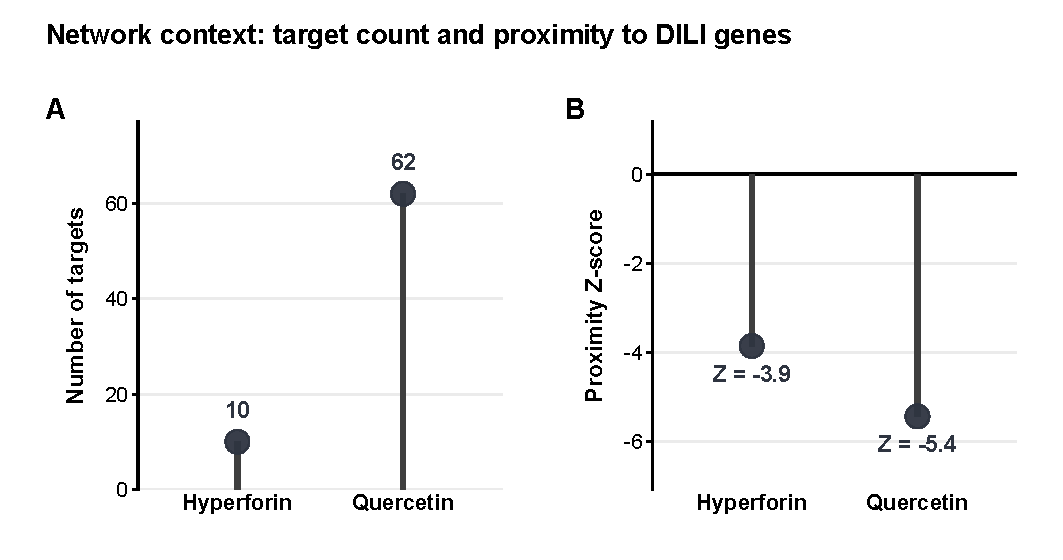
\includegraphics[width=\textwidth]{figures/fig1_lollipop.pdf}
\caption{\textbf{Network context.} Target count and shortest-path proximity ($d_c$) of Hyperforin (10 targets) and Quercetin (62 targets) to the 82-gene DILI module. Proximity Z-scores are deviations from a degree-matched null ($n=1{,}000$); negative values indicate closer-than-random proximity. STRING v12.0 ($\geq$900), GTEx v8 liver LCC.}
\label{fig:context}
\end{figure}

\begin{figure}[ht]
\centering
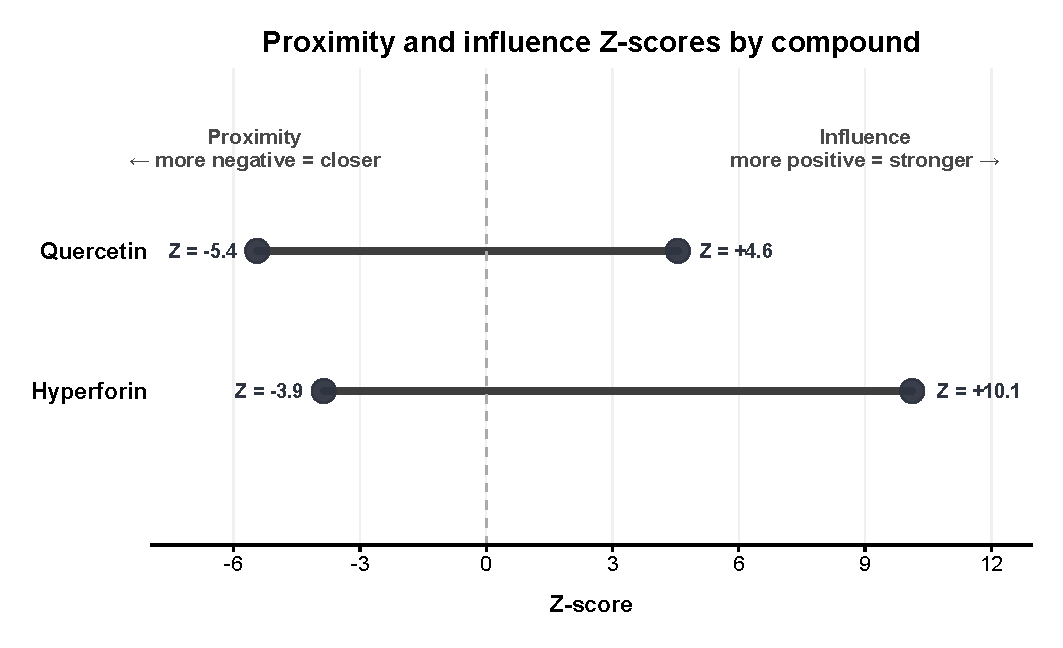
\includegraphics[width=0.85\textwidth]{figures/fig2_dumbbell.pdf}
\caption{\textbf{Effect size and evidence dissociate.} At STRING $\geq$900, Hyperforin is closer to the DILI module ($d_c=1.30$ vs $1.68$) yet has the weaker proximity Z-score ($-3.86$ vs $-5.44$); per-target influence ranks Hyperforin higher. Lines connect each compound's proximity and influence statistics. Degree-matched permutation nulls ($n=1{,}000$).}
\label{fig:dumbbell}
\end{figure}

\begin{figure}[ht]
\centering

\includegraphics[width=\textwidth]{figures/fig8_opregime.pdf}
\caption{\textbf{The null-precision law defines a conditional operating regime for rank reversal.} Degree-controlled target-set probes on the liver LCC and DILI module (Methods); no toxicity outcome is modelled. \textbf{(A)}~The null standard deviation scales as $\sigma_{\text{null}}\propto|T|^{-1/2}$ on the real DILI module (fitted slope $-0.50$; dashed $-1/2$ reference); the same exponent holds for random size-matched pseudo-modules (Table~\ref{tab:s_opregime}). \textbf{(B)}~The maximum raw-distance margin the larger set can overturn, $\delta_{\max}(R)$, increases with target-count ratio but saturates for fixed smaller-set size; the Hyperforin/Quercetin observed margin ($0.38$ at $R=6.2$) lies below the envelope and is therefore overturnable. \textbf{(C)}~Operating-regime plane at $R=6.2$: each point is a probe pair, plotted by raw-distance margin ($>0$: smaller set closer) versus evidence gap ($>0$: larger set stronger); the reversal region is shaded. Material-margin reversals are rare for generic probes; Hyperforin/Quercetin (orange) sits in the reversal region at the $91$st proximity percentile.}
\label{fig:opregime}
\end{figure}

\begin{figure}[ht]
\centering
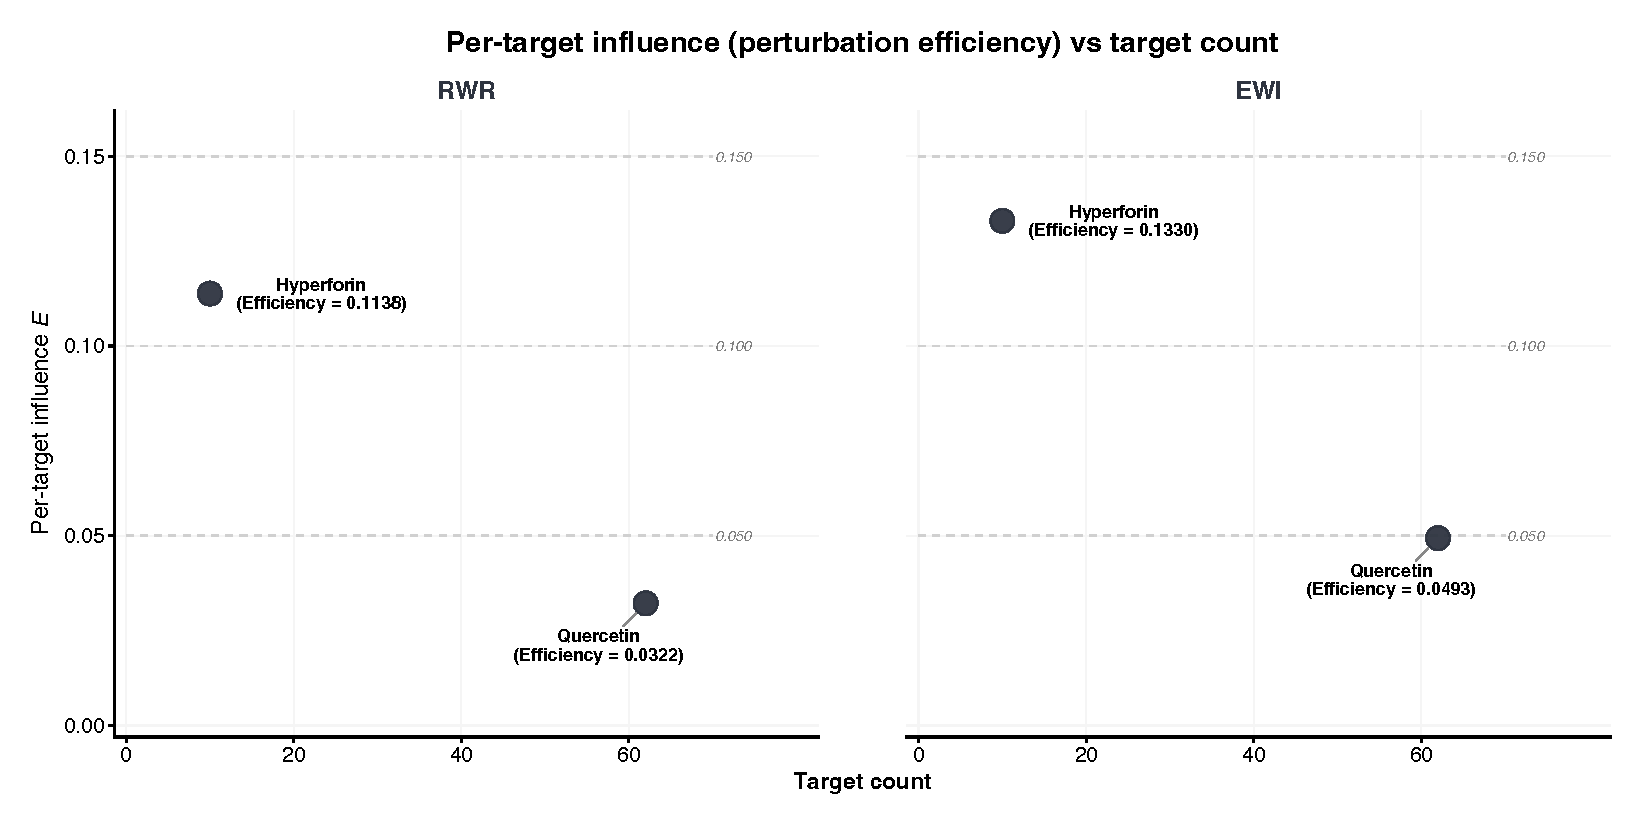
\includegraphics[width=\textwidth]{figures/fig4_ptni_phase.pdf}
\caption{\textbf{Perturbation efficiency.} Per-target influence (perturbation efficiency $E$, Eq.~\eqref{eq:pe}) versus target count; horizontal lines mark constant-influence tiers. $E$ is the mean per-target influence on the DILI module and is comparable across compounds of different target count.}
\label{fig:efficiency}
\end{figure}

\begin{figure}[ht]
\centering
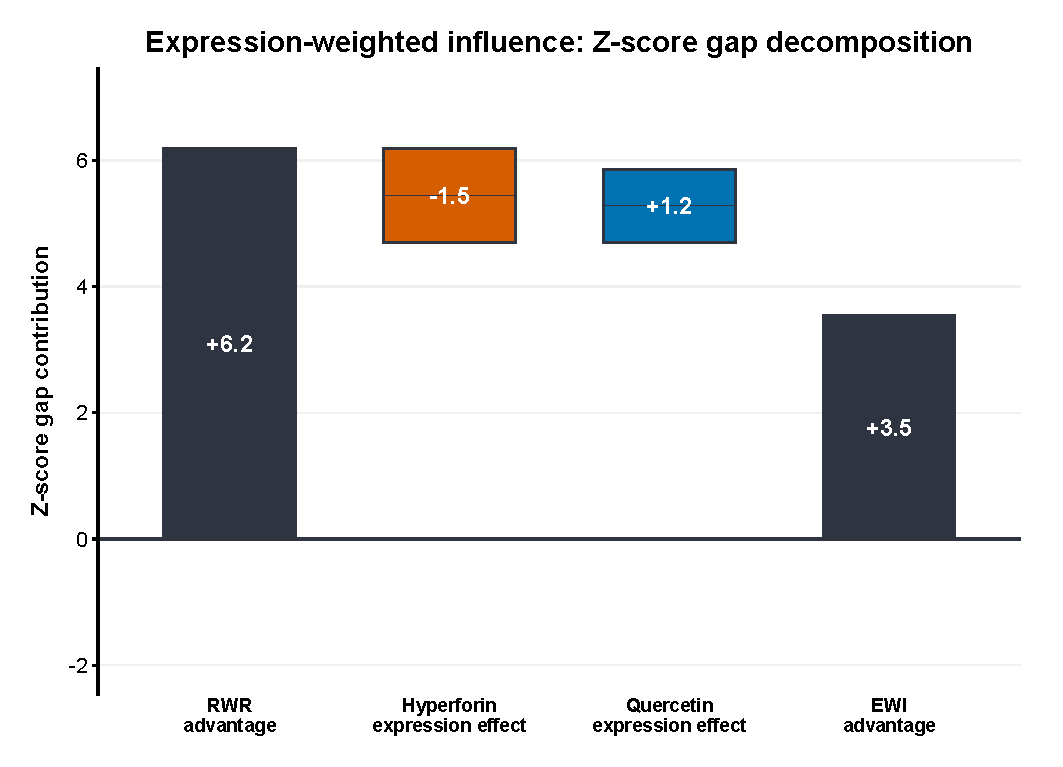
\includegraphics[width=0.9\textwidth]{figures/fig3_ewi_waterfall.pdf}
\caption{\textbf{Expression-weighted influence.} Waterfall decomposition of the RWR Z-score gap (Hyperforin $-$ Quercetin) under destination-node liver-expression weighting: the gap narrows from $+6.19$ (RWR) to $+3.54$ (EWI). Hyperforin attenuates ($-1.49$ contribution to the gap), while Quercetin gains $+1.16$ in its own Z-score, corresponding to a $-1.16$ contribution to the Hyperforin-minus-Quercetin gap; the ranking persists and is insensitive to the expression floor. GTEx v8 liver, STRING $\geq$900, $n=1{,}000$.}
\label{fig:ewi}
\end{figure}

\begin{figure}[ht]
\centering
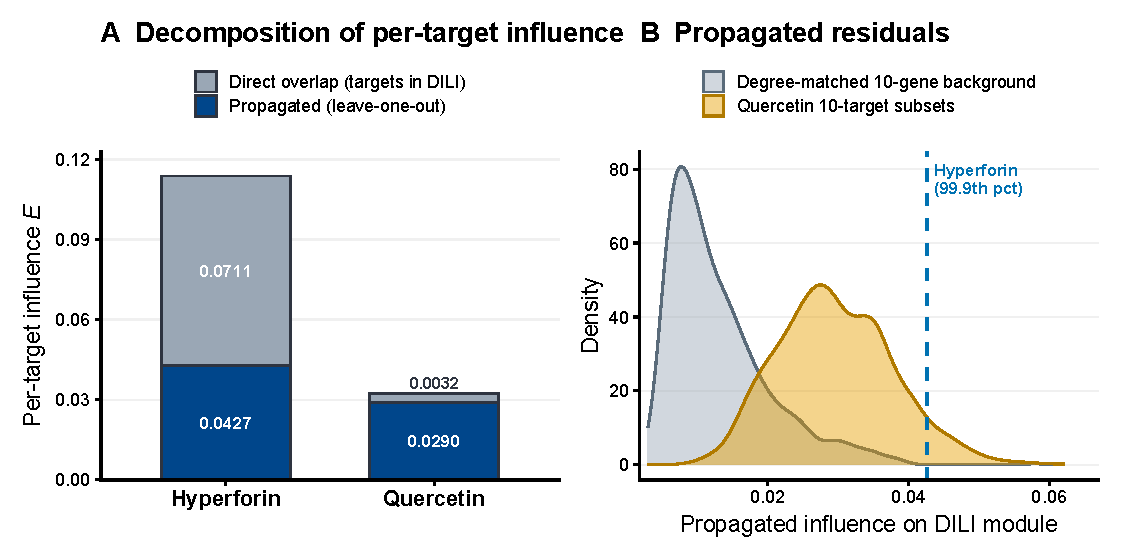
\includegraphics[width=\textwidth]{figures/fig7_leakage.pdf}
\caption{\textbf{Direct versus propagated decomposition of per-target influence} (STRING $\geq$900). \textbf{(A)}~Per-target influence $E$ separates into a direct-overlap component (steady-state mass on target$\cap$DILI nodes) and a propagated component isolated by leave-one-out; 62\% of Hyperforin's influence is direct overlap, and the two compounds' propagated components are close (0.0427 vs 0.0290). \textbf{(B)}~The propagated component against null models: Hyperforin (dashed line, 99.9th percentile) exceeds a degree-matched random 10-gene background but lies within the spread of size-matched Quercetin 10-target subsets ($n=1{,}000$ each), indicating an above-background but non-unique propagated residual.}
\label{fig:leakage}
\end{figure}

\begin{figure}[ht]
\centering

\includegraphics[width=0.65\textwidth]{figures/fig6_chemsim.pdf}
\caption{\textbf{Chemical-similarity control.} Maximum Tanimoto similarity to DILIrank 2.0 reference drugs (retrievable-SMILES binary subset: 542 DILI-positive [vMost/vLess-concern] and 365 DILI-negative [vNo-concern]; 354 ambiguous-concern drugs excluded); both compounds fall below the 0.4 structural-analogue threshold, arguing against close structural confounding within the DILIrank reference set.}
\label{fig:chemsim}
\end{figure}

\clearpage
\begin{center}
{\Large\textbf{Supplementary Information}}\\[1em]
{\large Separating effect size from statistical evidence in network-proximity rankings under target-count asymmetry}\\[1em]
\suppauthor
\end{center}
\vspace{1.5em}

\setcounter{table}{0}
\renewcommand{\thetable}{S\arabic{table}}
\setcounter{figure}{0}
\renewcommand{\thefigure}{S\arabic{figure}}

\section*{Supplementary Notes}

\textbf{Network type.} STRING combined-confidence edges integrate multiple evidence channels (experiments, curated databases, co-expression, genomic context, text mining); the resulting graph is a \textit{functional association network}, not a purely physical protein--protein binding network. We use ``interactome'' in this broad STRING association-network sense throughout.

\textbf{Text-mining robustness.} Because the DILI module is DisGeNET-derived (literature-based) and the STRING combined score includes a text-mining channel, some target--DILI edges could reflect literature co-mention rather than independent evidence. Following \citet{Huang2018}, we rebuilt the interactome after removing every edge supported \textit{solely} by the STRING text-mining channel (all other evidence channels zero) and re-ran all three metrics; a from-scratch rebuild without this filter recovers all committed network edges (0 missing, with a small mapping superset), and the full-rebuild observed values match the committed values, so the comparison is mapping-consistent. Text-mining-only edges constitute 0.7\% ($\geq$900) to 2.4\% ($\geq$700) of the liver-expressed LCC. Removing them leaves the effect ordering intact: Hyperforin remains closer ($d_c=1.30$ vs $1.67$ at $\geq$900) and higher in per-target random-walk ($0.114$ vs $0.033$) and expression-weighted ($0.134$ vs $0.050$) influence, with the ordering preserved on all three metrics at both thresholds (all $p<0.002$; per-metric values in Table~\ref{tab:s_textmining}, full output in \texttt{results/tables/string\_textmining\_sensitivity.csv}). This argues against literature text-mining circularity as the driver of the effect/evidence dissociation, consistent with \citeauthor{Huang2018}'s finding that STRING's disease-gene signal is robust to text-mining removal.

\textbf{DILI-module provenance.} The DILI gene set is derived from DisGeNET curated gene--disease associations (UMLS C0860207). It is a \textit{curated association module}, not a validated causal gene set: some members are metabolism genes, pharmacogenes, or literature-associated biomarkers rather than established causal DILI drivers. This is relevant because four Hyperforin targets (NR1I2, CYP2C9, ABCB1, MMP2) are themselves members of this module; the direct--propagated decomposition (Table~\ref{tab:s_leak}) quantifies the resulting direct overlap.

\textbf{Null estimands.} Two degree-matched permutation nulls are reported. The \textit{fixed-disease null} randomises only the target set and holds the disease module at the 82 real DILI genes; it answers ``are these targets unusually close to \textit{this} disease module?'' and is the appropriate primary null for comparing two compounds against the same disease. The \textit{two-sided null} (after \citet{Guney2016}) additionally randomises a degree-matched disease set; it answers the population-level drug--disease question and is reported as a fidelity sensitivity (Table~\ref{tab:s_guney}).

\textbf{p-value convention.} All permutation p-values are empirical, directional, and computed as $(r+1)/(n+1)$ \citep{Phipson2010}: one-sided for \textit{smaller-than-null distance} (proximity) and \textit{larger-than-null influence} (RWR/EWI). With $n=1{,}000$ the floor is $9.99\times10^{-4}$. Z-scores are the primary magnitude report; no two-tailed permutation p-value is used.

\section*{Supplementary Figures}

\begin{figure}[ht]
\centering
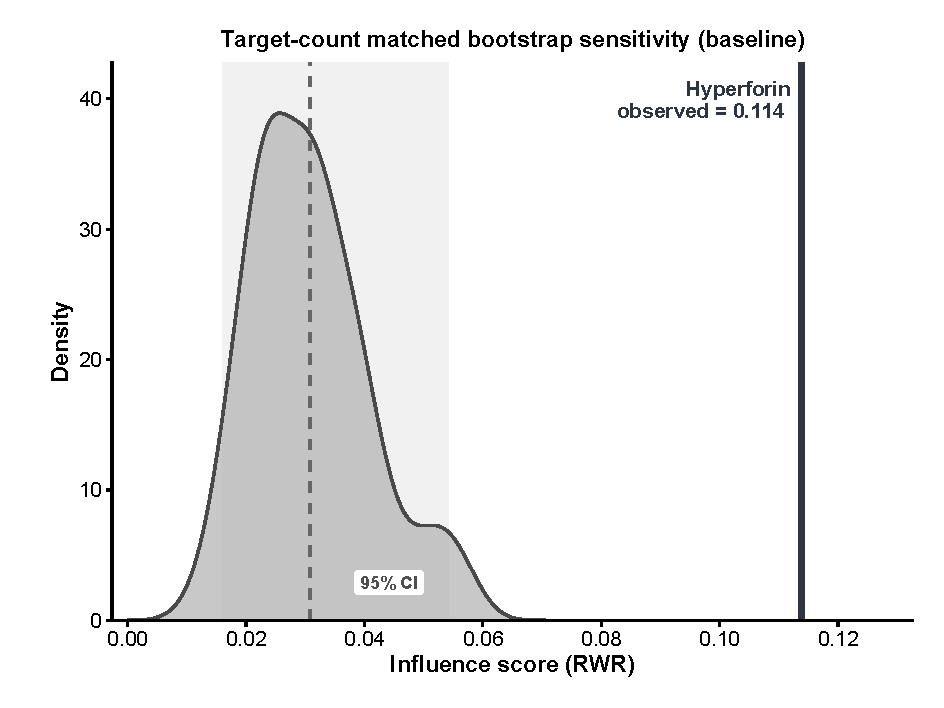
\includegraphics[width=0.7\textwidth]{figures/fig5_bootstrap.pdf}
\caption{\textbf{Bootstrap sensitivity (baseline).} Distribution of RWR influence for random 10-target subsets of Quercetin; solid line, Hyperforin observed influence. This baseline control does not adjust for target--DILI overlap; the leakage-controlled analysis (Table~\ref{tab:leakage}, Fig.~\ref{fig:leakage}) supersedes the headline ratio. STRING $\geq$900.}
\label{fig:bootstrap}
\end{figure}

\section*{Supplementary Tables}

% S1: Target-evidence table
\begin{table}[ht]
\centering
\caption{\textbf{Target curation evidence.} Hyperforin targets are literature-curated and span a direct nuclear receptor (PXR/NR1I2), PXR-induced downstream enzymes, transporters, and direct-inhibition targets; Quercetin targets are uniformly ChEMBL bioactivity-derived. This documents the evidentiary asymmetry whose downstream consequence is audited in Table~\ref{tab:s_leak}.}
\label{tab:s_evidence}
\small
\begin{tabular}{@{}llllccc@{}}
\toprule
\textbf{Gene} & \textbf{Source} & \textbf{Evidence type} & \textbf{Direct} & \textbf{In DILI} & \textbf{Shared} & \textbf{Kept$^\dagger$} \\
\midrule
\multicolumn{7}{l}{\textit{Hyperforin (literature-curated)}}\\
NR1I2  & literature & direct receptor agonist (PXR) & yes     & yes & no  & yes \\
CYP3A4 & literature & PXR-induced enzyme            & no      & no  & yes & no  \\
CYP2C9 & literature & enzyme (inhib./induction)     & partial & yes & no  & no  \\
CYP2B6 & literature & PXR-induced enzyme            & no      & no  & no  & no  \\
ABCB1  & literature & transporter (induced + inhib.)& yes     & yes & no  & no  \\
ABCG2  & literature & transporter modulation        & partial & no  & yes & no  \\
ABCC2  & literature & transporter modulation        & partial & no  & no  & no  \\
AKT1   & literature & direct kinase inhibition      & yes     & no  & yes & yes \\
MMP2   & literature & secretion inhibition          & partial & yes & yes & yes \\
MMP9   & literature & secretion inhibition          & partial & no  & yes & yes \\
\addlinespace
\multicolumn{7}{l}{\textit{Quercetin (ChEMBL bioactivity, CHEMBL159; 62 targets, full list Table~\ref{tab:s_quer})}}\\
\multicolumn{3}{l}{in vitro binding/activity (IC$_{50}$/K$_i$/EC$_{50}\leq$10\,$\mu$M)} & yes & MMP2 (1) & 5 & n/a \\
\bottomrule
\end{tabular}

\vspace{0.3em}
\begin{minipage}{\linewidth}\footnotesize ``Direct'' classifies the target--compound interaction: \textit{yes} = direct molecular target (receptor agonism or enzyme/kinase inhibition); \textit{partial} = mixed or context-dependent direct engagement (e.g.\ both induction and inhibition); \textit{no} = downstream induced effect rather than direct binding. $^\dagger$Kept = retained in the ``CYP/transporter-out'' leakage control (Table~\ref{tab:s_leak}).\end{minipage}
\end{table}

% S2: Hyperforin targets with CORRECTED degrees
\begin{table}[ht]
\centering
\caption{\textbf{Hyperforin targets in the liver-expressed LCC} (STRING $\geq$900). Node degrees are recomputed in the analysis network (correcting earlier values taken from a larger network). TPM from GTEx v8 liver.}
\label{tab:s_hyptargets}
\begin{tabular}{@{}llrrl@{}}
\toprule
\textbf{Gene} & \textbf{Protein} & \textbf{TPM} & \textbf{Degree} & \textbf{DILI link} \\
\midrule
NR1I2  & PXR         & 43  & 4   & direct (module member) \\
CYP3A4 & CYP3A4      & 335 & 73  & indirect \\
CYP2C9 & CYP2C9      & 434 & 52  & direct (module member) \\
CYP2B6 & CYP2B6      & 125 & 34  & indirect \\
AKT1   & PKB         & 33  & 128 & indirect \\
ABCB1  & P-gp        & 7   & 1   & direct (module member) \\
ABCC2  & MRP2        & 60  & 1   & indirect \\
ABCG2  & BCRP        & 4   & 2   & indirect \\
MMP2   & MMP-2       & 5   & 20  & direct (module member) \\
MMP9   & MMP-9       & 1   & 25  & indirect \\
\bottomrule
\end{tabular}
\end{table}

% (former null-SD-by-|T| table removed here: it duplicated main-text Table~2 verbatim;
%  the per-metric null parameters are tabulated below.)

% S-null: permutation null parameters by metric (Reviewer-2-referenced table)
\begin{table}[ht]
\centering
\caption{\textbf{Permutation null parameters across metrics} (STRING $\geq$900; $n=1{,}000$ degree-matched permutations). The null standard deviation $\sigma_{\text{null}}$ of the 62-target compound is $\approx$2.5$\times$ smaller than that of the 10-target compound for shortest-path, random-walk \emph{and} expression-weighted influence alike --- the Law-of-Large-Numbers shrinkage ($\sqrt{62/10}=2.49$), identical across metrics. This is why Z-score magnitude is not comparable across compounds of very different target count.}
\label{tab:s_nullsd}
\begin{tabular}{@{}ll S[table-format=1.4] S[table-format=1.4] S[table-format=1.4] S[table-format=+2.2]@{}}
\toprule
\textbf{Metric} & \textbf{Compound} & {$\mu_{\text{null}}$} & {$\sigma_{\text{null}}$} & {$x_{\text{obs}}$} & {$Z$} \\
\midrule
Shortest-path $d_c$ & Hyperforin (10) & 2.2086 & 0.2353 & 1.3000 & -3.86 \\
                    & Quercetin (62)  & 2.1749 & 0.0914 & 1.6774 & -5.44 \\
\addlinespace
RWR influence       & Hyperforin (10) & 0.0141 & 0.0093 & 0.1138 & +10.77 \\
                    & Quercetin (62)  & 0.0148 & 0.0038 & 0.0322 & +4.58 \\
\addlinespace
EWI influence       & Hyperforin (10) & 0.0196 & 0.0122 & 0.1330 & +9.28 \\
                    & Quercetin (62)  & 0.0210 & 0.0049 & 0.0493 & +5.74 \\
\midrule
\multicolumn{6}{@{}l}{\footnotesize $\sigma_{\text{null}}$ ratio (Hyperforin/Quercetin): shortest-path 2.57, RWR 2.45, EWI 2.47 (expected $\sqrt{62/10}=2.49$).}\\
\bottomrule
\end{tabular}
\end{table}

% S-opregime: operating-regime reversal rates
\begin{table}[ht]
\centering
\caption{\textbf{Operating-regime benchmark: margin-conditional rank-reversal rates} (liver LCC $\geq$900, DILI module; probes pinned to the full compound-target row degree profile, with DILI-module genes excluded from the candidate pool; smaller set $|T_S|=10$; $500{,}000$ probe pairs per row, seed 42). Each entry is the fraction of pairs in which the smaller set is genuinely closer by a material raw margin ($\geq\delta_0$ hops) yet the larger set has the more negative Z-score. Reversals are rare and require a smaller set above the 90th percentile of probe-pair margins: a no-shrinkage counterfactual ($\sigma_L:=\sigma_S$) gives $0\%$ at every $R$, and unconditionally the Hyperforin/Quercetin directional pattern (smaller set closer \emph{and} larger set stronger Z) occurs in only $6.5\%$ of exact $R=6.2$ pairs, collapsing to near-zero once a material margin is required. The null-SD exponent is $-0.499$ (95\% CI $[-0.502,-0.495]$, $R^2=0.9999$) and similar across the DILI module and three size-matched pseudo-modules (DILI $-0.495$; three random size-matched pseudo-modules mean $-0.498$).}
\label{tab:s_opregime}
\begin{tabular}{@{}cc S[table-format=1.2] S[table-format=1.2]@{}}
\toprule
$R=|T_L|/|T_S|$ & $(|T_S|,|T_L|)$ & {reversal, $\delta_0\geq0.3$ (\%)} & {reversal, $\delta_0\geq0.5$ (\%)} \\
\midrule
1.5 & (10,\,15) & 0.00 & 0.00 \\
2.0 & (10,\,20) & 0.00 & 0.00 \\
3.0 & (10,\,30) & 0.00 & 0.00 \\
4.0 & (10,\,40) & 0.00 & 0.00 \\
6.0 & (10,\,60) & 0.10 & 0.00 \\
6.2 & (10,\,62) & 0.06 & 0.00 \\
8.0 & (10,\,80) & 0.39 & 0.00 \\
\bottomrule
\end{tabular}
\end{table}

% S-textmining: text-mining sensitivity values (before/after removing TM-only edges)
\begin{table}[ht]
\centering
\caption{\textbf{Text-mining robustness: metric values before and after removing text-mining-only STRING edges} (liver-expressed LCC; following \citet{Huang2018}, every edge supported \textit{solely} by the STRING text-mining channel was removed). ``Committed'' is the value in the main analysis; ``no-TM'' is after removal. The Hyperforin\,$>$\,Quercetin ordering (smaller $d_c$; larger influence) is preserved on all three metrics at both network thresholds, and every no-TM permutation $p<0.002$; arguing against literature text-mining circularity as the driver. Source: \texttt{results/tables/string\_textmining\_sensitivity.csv}.}
\label{tab:s_textmining}
\small
\begin{tabular}{@{}ll S[table-format=1.4] S[table-format=1.4] S[table-format=1.4] S[table-format=1.4] c@{}}
\toprule
& & \multicolumn{2}{c}{\textbf{Hyperforin}} & \multicolumn{2}{c}{\textbf{Quercetin}} & \\
\cmidrule(lr){3-4}\cmidrule(lr){5-6}
\textbf{Metric} & \textbf{STRING} & {committed} & {no-TM} & {committed} & {no-TM} & \textbf{winner} \\
\midrule
$d_c$ (smaller closer) & $\geq$700 & 0.6000 & 0.6000 & 1.3387 & 1.3387 & Hyp \\
                       & $\geq$900 & 1.3000 & 1.3000 & 1.6774 & 1.6721 & Hyp \\
\addlinespace
RWR influence (larger) & $\geq$700 & 0.1212 & 0.1243 & 0.0326 & 0.0335 & Hyp \\
                       & $\geq$900 & 0.1138 & 0.1144 & 0.0322 & 0.0329 & Hyp \\
\addlinespace
EWI influence (larger) & $\geq$700 & 0.1449 & 0.1472 & 0.0511 & 0.0516 & Hyp \\
                       & $\geq$900 & 0.1330 & 0.1337 & 0.0493 & 0.0501 & Hyp \\
\bottomrule
\end{tabular}
\end{table}

% S4: threshold robustness (>=700 vs >=900)
\begin{table}[ht]
\centering
\caption{\textbf{Threshold robustness} (STRING $\geq$700 vs $\geq$900 liver LCC; $n=1{,}000$, seed 42). The proximity-Z \emph{ranking} reverses across thresholds --- Hyperforin is the more ``significant'' at $\geq$700, Quercetin at $\geq$900 --- whereas the raw closest distance ($d_c$, Hyperforin closer) and the per-target influence ($E$, Hyperforin higher) rankings are stable at both thresholds. This is the effect-size/evidence dissociation of the main text, shown across network construction.}
\label{tab:s_threshold}
\begin{tabular}{@{}llcccc@{}}
\toprule
& & \multicolumn{2}{c}{\textbf{STRING $\geq$700}} & \multicolumn{2}{c}{\textbf{STRING $\geq$900}} \\
\cmidrule(lr){3-4}\cmidrule(lr){5-6}
\textbf{Metric} & \textbf{Compound} & value & $Z$ & value & $Z$ \\
\midrule
$d_c$ (closest distance) & Hyperforin & 0.60 & $-6.04$ & 1.30 & $-3.86$ \\
                         & Quercetin  & 1.34 & $-5.46$ & 1.68 & $-5.44$ \\
\addlinespace
$E$ (RWR influence)      & Hyperforin & 0.1212 & $+11.04$ & 0.1138 & $+10.77$ \\
                         & Quercetin  & 0.0326 & $+5.46$  & 0.0322 & $+4.58$ \\
\addlinespace
$E$ (EWI influence)      & Hyperforin & 0.1449 & $+10.35$ & 0.1330 & $+9.28$ \\
                         & Quercetin  & 0.0511 & $+7.01$  & 0.0493 & $+5.74$ \\
\bottomrule
\end{tabular}
\end{table}

% S5: alpha sweep
\begin{table}[ht]
\centering
\caption{\textbf{Restart-probability ($\alpha$) sensitivity} (STRING $\geq$900). The Hyperforin $>$ Quercetin per-target-efficiency ranking holds at every $\alpha$; the ratio is $\alpha$-dependent and is not interpreted as an absolute constant.}
\label{tab:s_alpha}
\begin{tabular}{@{}lcccccc@{}}
\toprule
$\alpha$ & 0.10 & 0.15 & 0.20 & 0.30 & 0.50 & 0.70 \\
\midrule
$E$ Hyperforin & 0.0907 & 0.1138 & 0.1344 & 0.1716 & 0.2390 & 0.3032 \\
$E$ Quercetin  & 0.0312 & 0.0322 & 0.0322 & 0.0310 & 0.0271 & 0.0227 \\
ratio          & 2.90 & 3.54 & 4.18 & 5.53 & 8.81 & 13.35 \\
\bottomrule
\end{tabular}
\end{table}

% S5: floor sweep
\begin{table}[ht]
\centering
\caption{\textbf{Expression-floor sensitivity (EWI)} (STRING $\geq$900). The 0.01 floor is immaterial; the ratio moves only in the third decimal.}
\label{tab:s_floor}
\begin{tabular}{@{}lccccc@{}}
\toprule
floor & 0 & $10^{-3}$ & $10^{-2}$ & $5\times10^{-2}$ & $10^{-1}$ \\
\midrule
$E$ Hyperforin & 0.1330 & 0.1330 & 0.1330 & 0.1330 & 0.1327 \\
$E$ Quercetin  & 0.0493 & 0.0493 & 0.0493 & 0.0493 & 0.0491 \\
ratio          & 2.695 & 2.695 & 2.695 & 2.695 & 2.702 \\
\bottomrule
\end{tabular}
\end{table}

% S6: direct-propagated decomposition (full controls)
\begin{table}[ht]
\centering
\caption{\textbf{Direct--propagated decomposition of per-target influence: full controls} (STRING $\geq$900). Four of ten Hyperforin targets are DILI-module members vs one of 62 Quercetin targets; isolating the propagated component (leave-one-out) and removing each source of direct overlap attenuates the per-target advantage to a modest residual.}
\label{tab:s_leak}
\begin{tabular}{@{}p{0.36\textwidth}ccc@{}}
\toprule
\textbf{Control} & \textbf{$E$(Hyp)} & \textbf{$E$(Quer)} & \textbf{ratio} \\
\midrule
Baseline (includes overlap) & 0.1138 & 0.0322 & 3.54 \\
Self-mass excluded & 0.0427 & 0.0290 & 1.47 \\
DILI-member seeds removed & 0.0431 & 0.0295 & 1.46 \\
CYP/transporter seeds removed & 0.0338 & 0.0290 & 1.17 \\
Shared targets removed (both) & 0.0541 & 0.0288 & 1.88 \\
\midrule
\multicolumn{4}{@{}p{0.95\textwidth}@{}}{\textit{Propagated (leave-one-out) reference distributions ($n=1{,}000$; Fig.~\ref{fig:leakage}B):}}\\
Global degree-matched random set ($n=10$) & \multicolumn{3}{p{0.52\textwidth}@{}}{Hyp 0.0427 vs null mean 0.0130 (95th 0.0281; max 0.0580); 99.9th percentile, 3.3$\times$ mean, $p=0.002$, does not exceed all}\\
Size-matched Quercetin 10-subsets & \multicolumn{3}{p{0.52\textwidth}@{}}{Hyp 0.0427 vs subset mean 0.0296 (max 0.0622); 1.4$\times$, overlapping}\\
\bottomrule
\end{tabular}
\end{table}

% S7: separation measure (Menche 2015)
\begin{table}[ht]
\centering
\caption{\textbf{Network separation between target set and DILI module.} Menche et al.\ separation measure $S_{AB}=\langle d_{AB}\rangle-(\langle d_{AA}\rangle+\langle d_{BB}\rangle)/2$ \citep{Menche2015} (STRING $\geq$900); $S_{AB}>0$ indicates topological separation. Both target sets are separated from the DILI module, and Hyperforin is \emph{more} separated despite its four direct-overlap targets, because its targets form a tighter cluster ($\langle d_{AA}\rangle=1.20$ vs $1.55$). This corroborates the decomposition (Table~\ref{tab:leakage}, Fig.~\ref{fig:leakage}): Hyperforin's per-target influence advantage arises from a few targets that \emph{are} DILI genes (direct overlap), not from its target set being embedded in the DILI neighbourhood.}
\label{tab:s_sep}
\begin{tabular}{@{}l S[table-format=1.3] S[table-format=1.3] S[table-format=1.3] S[table-format=+1.3]@{}}
\toprule
\textbf{Target set} & {$\langle d_{AB}\rangle$} & {$\langle d_{AA}\rangle$} & {$\langle d_{BB}\rangle$} & {$S_{AB}$} \\
\midrule
Hyperforin & 1.699 & 1.200 & 1.500 & +0.349 \\
Quercetin  & 1.644 & 1.548 & 1.500 & +0.119 \\
\bottomrule
\end{tabular}
\end{table}

% S-connectivity: direct (distance-1) DILI connectivity (regenerated on >=900 LCC)
\begin{table}[ht]
\centering
\caption{\textbf{Direct (distance-1) DILI connectivity of Hyperforin targets} (regenerated on the STRING $\geq$900 liver LCC). Connectivity is concentrated in the cytochrome-P450 axis; the transporters (ABCB1, ABCC2, ABCG2) and the receptor NR1I2 have no additional distance-1 DILI neighbours (NR1I2 and ABCB1 are themselves module members, at distance 0). Per-target means: \textbf{Hyperforin 3.40} direct DILI neighbours (34 connections across 10 targets) vs \textbf{Quercetin 1.53} (95 across 62) --- a $2.2\times$ enrichment that complements the distance-0 direct-overlap decomposition (Table~\ref{tab:s_leak}).}
\label{tab:s_connectivity}
\footnotesize
\begin{tabular}{@{}lcp{9.4cm}@{}}
\toprule
\textbf{Hyperforin target} & \textbf{$n$} & \textbf{Direct DILI neighbours (distance 1)} \\
\midrule
CYP3A4 & 11 & CYP2A6, CYP2C19, CYP2C9, CYP2E1, FMO3, GSTM1, GSTM2, GSTP1, NR1I2, NR1I3, UGT1A9 \\
CYP2C9 & 9  & CYP2A6, CYP2C19, CYP2E1, FMO3, GSTM1, GSTM2, GSTP1, PTGS2, UGT1A9 \\
CYP2B6 & 6  & CYP2A6, CYP2C19, CYP2C9, CYP2E1, PTGS2, UGT1A9 \\
AKT1   & 4  & CTNNB1, IGF1, MAP3K5, NFE2L2 \\
MMP9   & 3  & LCN2, MMP2, SPP1 \\
MMP2   & 1  & LCN2 \\
ABCB1, ABCC2, ABCG2, NR1I2 & 0 & --- \\
\bottomrule
\end{tabular}
\end{table}

% S-modulesens: DILI-module sensitivity (remove entangled pharmacogenes from the module)
\begin{table}[ht]
\centering
\caption{\textbf{DILI-module sensitivity: removing the entangled pharmacogenes.} Every other robustness check in this work varies the \emph{method} ($\alpha$, expression floor, network threshold, degree-binning, two nulls); this one varies the \emph{disease module}, the locus of the target--disease circularity. We remove from the 82-gene module the four genes that are simultaneously Hyperforin targets and DILI members (ABCB1, CYP2C9, MMP2, NR1I2), giving a reduced module $D'$ that the drug targets cannot directly overlap, and recompute the propagated (leave-one-out) per-target influence symmetrically for both compounds (STRING $\geq$900, $\alpha=0.15$). The propagated advantage does \emph{not} collapse --- it slightly increases, because Hyperforin's leave-one-out value is unchanged (those genes were already excluded from its own scoring) while Quercetin loses propagation onto ABCB1/CYP2C9/NR1I2, which it had benefited from as non-target DILI genes. Against a degree-matched random 10-gene background scored on $D'$ ($n=1{,}000$), Hyperforin remains at the 99th percentile ($3.45\times$ the background mean, empirical $p=0.005$) but does not exceed every random set. The modest propagated signal supports the interpretation that the propagated residual is not eliminated after removing the overlapping pharmacogenes from the module.}
\label{tab:s_modulesens}
\begin{tabular}{@{}l S[table-format=2.0] S[table-format=1.4] S[table-format=1.4] S[table-format=1.2]@{}}
\toprule
\textbf{Disease module} & {$|D|$} & {Propagated $E$ (Hyp)} & {Propagated $E$ (Quer)} & {Ratio} \\
\midrule
Full DILI module            & 82 & 0.0427 & 0.0290 & 1.47 \\
Overlap genes removed ($D'$) & 78 & 0.0427 & 0.0271 & 1.58 \\
\bottomrule
\end{tabular}
\end{table}

% S10: Guney fidelity -- full null parameters (expanded companion to main-text Table tab:guney)
\begin{table}[ht]
\centering
\caption{\textbf{Independent reimplementation of the canonical proximity toolbox: full null parameters} (\texttt{emreg00/toolbox}, re-derived by \texttt{GUNEY\_FIDELITY\_check.py}; STRING $\geq$900; $n=1{,}000$; seed 42; $|D|=82$ preserved). This is the detailed companion to the compact main-text summary (Table~\ref{tab:guney}): for each null construction it reports the observed closest distance $d_c$, the null mean $\mu_{\text{null}}$ and standard deviation $\sigma_{\text{null}}$, and the resulting $Z$. The observed $d_c$ reproduces the toolbox exactly (Hyperforin 1.300, Quercetin 1.677). The reimplementation's $\pm$25\% window (group 1, Quercetin $Z=-5.35$) matches the committed \texttt{src} pipeline ($Z=-5.44$; Table~\ref{tab:s_nullsd}) within permutation tolerance, confirming the two implementations agree. The $\pm$25\% window never silently falls back to unmatched nodes: every Hyperforin target retains $\geq$143 degree-matched candidates (its highest-degree target, AKT1, has degree 128). The evidence dissociation is clear under the fixed-disease null and attenuates to near-parity under the two-sided null; Hyperforin is the topologically closer compound throughout.}
\label{tab:s_guney}
\begin{tabular}{@{}ll S[table-format=1.2] S[table-format=1.2] S[table-format=1.3] S[table-format=-1.2]@{}}
\toprule
\textbf{Null model} & \textbf{Compound} & {$d_c$} & {$\mu_{\text{null}}$} & {$\sigma_{\text{null}}$} & {$Z$} \\
\midrule
$\pm$25\% window, fixed disease & Hyperforin & 1.30 & 2.22 & 0.238 & -3.86 \\
                                & Quercetin  & 1.68 & 2.18 & 0.093 & -5.35 \\
\addlinespace
Guney $\geq$100-bin, fixed disease & Hyperforin & 1.30 & 2.23 & 0.228 & -4.09 \\
                                   & Quercetin  & 1.68 & 2.16 & 0.090 & -5.34 \\
\addlinespace
Guney $\geq$100-bin, two-sided & Hyperforin & 1.30 & 2.05 & 0.212 & -3.55 \\
                               & Quercetin  & 1.68 & 2.01 & 0.090 & -3.66 \\
\midrule
\multicolumn{6}{@{}p{0.92\textwidth}}{\footnotesize $\sigma_{\text{null}}$ ratio (Hyperforin/Quercetin), from full-precision values: 2.56 ($\pm$25\% fixed), 2.53 ($\geq$100-bin fixed), 2.37 ($\geq$100-bin two-sided); expected $\sqrt{62/10}=2.49$. The Law-of-Large-Numbers shrinkage therefore persists under every null construction, including Guney's exact two-sided null.}\\
\bottomrule
\end{tabular}
\end{table}

% S8: full Quercetin list
\begin{table}[ht]
\centering
\caption{\textbf{Quercetin target genes in the liver-expressed LCC} (STRING $\geq$900, GTEx v8 liver TPM $\geq$1; ChEMBL CHEMBL159). Sorted by descending TPM.}
\label{tab:s_quer}
\scriptsize
\begin{tabular}{lrlrlrlr}
\toprule
\textbf{Gene} & \textbf{TPM} & \textbf{Gene} & \textbf{TPM} & \textbf{Gene} & \textbf{TPM} & \textbf{Gene} & \textbf{TPM} \\
\midrule
CFB & 1115 & CYP3A4 & 335 & FN1 & 229 & ALDH2 & 183 \\
ANPEP & 160 & PPIA & 112 & SERPINA5 & 104 & CYP1A2 & 72 \\
CA2 & 64 & APP & 63 & PYGL & 55 & HDAC6 & 45 \\
ESRRA & 42 & MAOA & 35 & AKR1C2 & 33 & AKT1 & 33 \\
CTSH & 28 & XDH & 26 & CHRNA4 & 25 & PIK3R1 & 24 \\
PIM1 & 24 & LDLR & 23 & ELOVL1 & 18 & EGFR & 17 \\
PKN1 & 16 & GSK3A & 13 & YES1 & 13 & MET & 12 \\
DAPK1 & 12 & BACE1 & 11 & CSNK2A1 & 10 & FSTL1 & 9 \\
SIRT6 & 8 & GSK3B & 7 & CDK7 & 7 & CAV2 & 7 \\
PTPN2 & 6 & CYP1A1 & 5 & PRMT7 & 5 & MMP2 & 5 \\
AKR1B1 & 5 & PDE6D & 5 & BRAF & 4 & PTK2 & 4 \\
ABCG2 & 4 & IQGAP1 & 4 & ADRB2 & 3 & KDR & 3 \\
SRC & 3 & ALOX5 & 3 & CYP1B1 & 3 & TLR4 & 3 \\
NUAK1 & 3 & AXL & 2 & ADA & 2 & LCK & 2 \\
ABCC1 & 2 & PLK1 & 1 & ACHE & 1 & MMP9 & 1 \\
SYK & 1 & PDZK1IP1 & 1 & & & & \\
\bottomrule
\end{tabular}
\end{table}

% S-curation: curation provenance
\begin{table}[ht]
\centering
\caption{\textbf{Curation provenance} (stage counts, reproducible from the committed data). Targets are filtered to the intersection of the $\geq$700 and $\geq$900 liver LCCs, so target counts are identical at both thresholds; the DILI module is filtered per threshold.}
\label{tab:s_curation}
\begin{tabular}{@{}lrrr@{}}
\toprule
\textbf{Stage} & \textbf{Hyperforin} & \textbf{Quercetin} & \textbf{DILI module} \\
\midrule
Raw (lit. / ChEMBL / DisGeNET) & 14 & 122 & 127 \\
Processed (human, UniProt-mapped)              & 14 & 87  & --- \\
In $\geq$700 liver-expressed LCC               & 10 & 62  & 84 \\
In $\geq$900 liver-expressed LCC               & 10 & 62  & 82 \\
\bottomrule
\end{tabular}
\end{table}

% S-dili: full DILI gene list
\begin{table}[ht]
\centering
\caption{\textbf{DILI gene set (82 genes)} in the liver-expressed STRING $\geq$900 LCC (DisGeNET, UMLS C0860207; GTEx v8 liver TPM $\geq$1), alphabetical. The four genes that are also Hyperforin targets (the distance-0 direct overlap, Table~\ref{tab:s_leak}) are in bold.}
\label{tab:s_dili}
\scriptsize
\begin{tabular}{llllllll}
\toprule
\multicolumn{8}{c}{\textbf{82 DILI-associated genes}} \\
\midrule
\textbf{ABCB1} & AHR & ALB & ALDOB & AMBP & APOA1 & APOE & APOH \\
ARG1 & ARNT & ATG5 & BAX & BTD & C3 & CAT & CCL2 \\
CLU & COL3A1 & CTNNB1 & CXCL1 & CXCL10 & CYP2A6 & CYP2C19 & \textbf{CYP2C9} \\
CYP2E1 & DGAT2 & ENO1 & FGA & FLT1 & FMO3 & GADD45A & GC \\
GCLC & GPT & GSN & GSTM1 & GSTM2 & GSTP1 & HLA-A & HLA-B \\
HLA-DQB1 & HLA-DRB1 & HMGB1 & HMOX1 & HPD & HPX & IGF1 & IL18 \\
IL1R2 & KRT18 & LCN2 & LGALS3 & MAP3K5 & MED1 & \textbf{MMP2} & MTHFR \\
NAT2 & NFE2L2 & NR1H3 & NR1H4 & \textbf{NR1I2} & NR1I3 & PLAT & PLG \\
PNP & POLG & PON1 & PPARA & PRKDC & PTGS2 & RBP1 & SLPI \\
SNX18 & SOD1 & SOD3 & SPP1 & TALDO1 & TBXA2R & TCTN1 & TF \\
TTR & UGT1A9 & & & & & & \\
\bottomrule
\end{tabular}
\end{table}

\noindent\footnotesize All values above are regenerated by the committed pipeline and reviewer-evidence scripts; cross-document numerical consistency is enforced by \texttt{verify\_numbers.py}.


\end{document}
